\section{RESULTS AND DISCUSSION}
\begin{figure}[h!] 
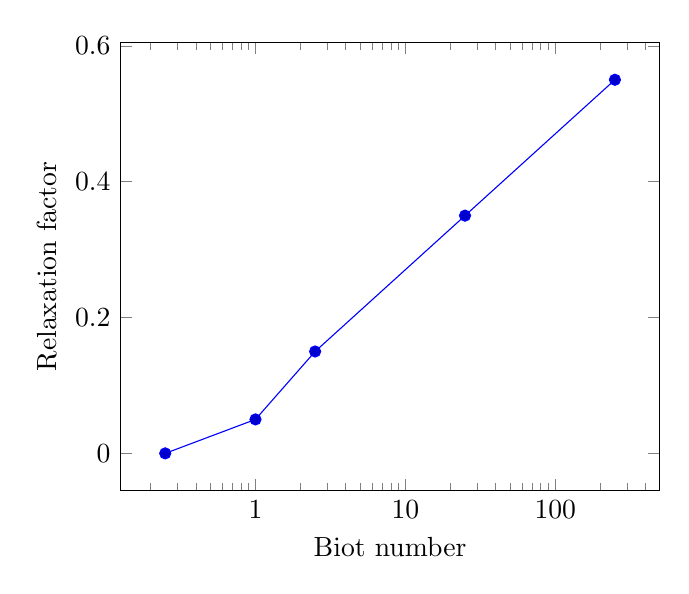
\begin{tikzpicture}
\begin{semilogxaxis}[
    unbounded coords=discard,
    log basis x=10,
    log ticks with fixed point
    ,xlabel=Biot number,ylabel=Relaxation factor]
\addplot coordinates {
(0.25,
0.00)
(1,
0.05)
(2.5,
0.15)
(25,
0.35)
(250,
0.55)
};
\end{semilogxaxis}
\end{tikzpicture}
  \caption{Relaxation needed as a function of the Biot number for the FFTB method and one Navier-Stokes solve per iteration. Biot number varied by means of the plate thickness.}
  \centering
\end{figure}